\documentclass[12pt, a4paper]{article}

% Required Packages
\usepackage{amsmath, graphicx}
\usepackage{amssymb}
\usepackage{kotex} % For Korean text
\usepackage{geometry}
\geometry{a4paper, margin=1in}
\graphicspath{{graph/}}
% Title

\title{Calculus - Chapter 9 Problems Plus (9.1 - 9.3)}
\author{}
\date{}

\begin{document}
\maketitle
\vspace{1em}
\begin{enumerate}
    \item Find all functions $f$ such that $f'$ is continuous and
    \[ [f(x)]^2 = 100 + \int_{0}^{x} \{[f(t)]^2 + [f'(t)]^2\} dt \]
    for all real $x$.
    \item Let $f$ be a function with the property that $f(0)=1, f'(0)=1$, and $f(a+b) = f(a)f(b)$ for all real numbers $a$ and $b$. Show that $f'(x) = f(x)$ for all $x$ and deduce that $f(x) = e^x$.

    \item A subtangent is a portion of the x-axis that lies directly beneath the segment of a tangent line from the point of contact to the x-axis. Find the curves that pass through the point $(c, 1)$ and whose subtangents all have length $c$.

    \item Find the curve that passes through the point (3, 2) and has the property that if the tangent line is drawn at any point P on the curve, then the part of the tangent line that lies in the first quadrant is bisected at P.

    \item Recall that the normal line to a curve at a point P on the curve is the line that passes through P and is perpendicular to the tangent line at P. Find the curve that passes through the point (3, 2) and has the property that if the normal line is drawn at any point on the curve, then the y-intercept of the normal line is always 6.

    \item Find all curves with the property that if the normal line is drawn at any point P on the curve, then the part of the normal line between P and the x-axis is bisected by the y-axis.

    \item Find all curves with the property that if a line is drawn from the origin to any point (x, y) on the curve, and then a tangent is drawn to the curve at that point and extended to meet the x-axis, the result is an isosceles triangle with equal sides meeting at (x, y).

    \begin{figure}[htbp] % [h!] 옵션은 여기에(here!) 그림을 위치시키라는 의미
        \centering % 이미지를 가운데로 정렬
       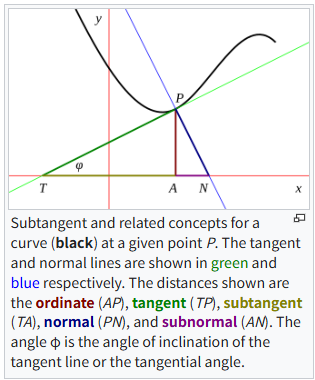
\includegraphics[width=0.4\textwidth]{graph7.png} % 너비는 텍스트 너비의 70%    
   \end{figure}

\end{enumerate}

\end{document}

